\documentclass[13pt,a4paper]{article}
\usepackage{a4wide,amssymb,epsfig,latexsym,multicol,array,hhline,fancyhdr}
\usepackage{vntex}
\usepackage{amsmath}
\usepackage{amsfonts}
\usepackage{lastpage}
\usepackage[lined,boxed,commentsnumbered]{algorithm2e}
\usepackage{enumerate}
\usepackage{color}
\usepackage{graphicx}							% Standard graphics package
\usepackage{array}
\usepackage{tabularx, caption}
\usepackage{multirow}
\usepackage{multicol}
\usepackage{rotating}
\usepackage{graphics}
\usepackage{geometry}
\usepackage{setspace}
\usepackage{subfig}
\usepackage{epsfig}
\usepackage{tikz}
\usepackage{listings}
\usepackage[
   sorting=none, 
	backend=biber,
	style=alphabetic,
]{biblatex}
\addbibresource{reference.bib}
\usetikzlibrary{arrows,snakes,backgrounds}
\usepackage{hyperref}
\hypersetup{urlcolor=blue,linkcolor=black,citecolor=black,colorlinks=true} 
%\usepackage{pstcol} 								% PSTricks with the standard color package

\newtheorem{theorem}{{\bf Theorem}}
\newtheorem{property}{{\bf Property}}
\newtheorem{proposition}{{\bf Proposition}}
\newtheorem{corollary}[proposition]{{\bf Corollary}}
\newtheorem{lemma}[proposition]{{\bf Lemma}}

\AtBeginDocument{\renewcommand*\contentsname{Mục lục}}
\AtBeginDocument{\renewcommand*\refname{Tài liệu tham khảo}}
%\usepackage{fancyhdr}
\setlength{\headheight}{40pt}
\pagestyle{fancy}
\fancyhead{} % clear all header fields
\fancyhead[L]{
	\begin{tabular}{rl}
		\begin{picture}(25,15)(0,0)
			\put(0,-8){
\includegraphics[width=8mm, height=8mm]{hcmut.png}}
			%\put(0,-8){\epsfig{width=10mm,figure=hcmut.eps}}
		\end{picture}&
		%
\includegraphics[width=8mm, height=8mm]{hcmut.png} & %
		\begin{tabular}{l}
			\textbf{\bf \ttfamily Trường Đại Học Bách Khoa TP. Hồ Chí Minh}\\
			\textbf{\bf \ttfamily Khoa Khoa Học Và Kĩ Thuật Máy Tính}
		\end{tabular} 	
	\end{tabular}
}
\fancyhead[R]{
	\begin{tabular}{l}
		\tiny \bf \\
		\tiny \bf 
\end{tabular}  }
\fancyfoot{} % clear all footer fields
\fancyfoot[L]{\scriptsize \ttfamily Báo cáo bài tập lớn 2 môn Hệ cơ sở dữ liệu (CO2013), HK1, năm học 2021-2022}
\fancyfoot[R]{\scriptsize \ttfamily Trang {\thepage}/\pageref{LastPage}}
\renewcommand{\headrulewidth}{0.3pt}
\renewcommand{\footrulewidth}{0.3pt}



%%%
\setcounter{secnumdepth}{4}
\setcounter{tocdepth}{3}
\makeatletter
\newcounter {subsubsubsection}[subsubsection]
\renewcommand\thesubsubsubsection{\thesubsubsection .\@alph\c@subsubsubsection}
\newcommand\subsubsubsection{\@startsection{subsubsubsection}{4}{\z@}%
	{-3.25ex\@plus -1ex \@minus -.2ex}%
	{1.5ex \@plus .2ex}%
	{\normalfont\normalsize\bfseries}}
\newcommand*\l@subsubsubsection{\@dottedtocline{3}{10.0em}{4.1em}}
\newcommand*{\subsubsubsectionmark}[1]{}
\makeatother

\definecolor{dkgreen}{rgb}{0,0.6,0}
\definecolor{gray}{rgb}{0.5,0.5,0.5}
\definecolor{mauve}{rgb}{0.58,0,0.82}
\lstset{frame=tb,
	language=Python,
	aboveskip=3mm,
	belowskip=3mm,
	showstringspaces=false,
	columns=flexible,
	basicstyle={\small\ttfamily},
	numbers=left,
	numberstyle=\tiny\color{gray},
	%identifierstyle=\color{purple}
	keywordstyle=\color{blue},
	commentstyle=\color{dkgreen},
	stringstyle=\color{mauve},
	breaklines=true,
	breakatwhitespace=true,
	tabsize=3
}

\begin{document}
	
	\begin{titlepage}
		\begin{center}
			ĐẠI HỌC QUỐC GIA THÀNH PHỐ HỒ CHÍ MINH \\
			TRƯỜNG ĐẠI HỌC BÁCH KHOA \\
			KHOA KHOA HỌC - KỸ THUẬT MÁY TÍNH
		\end{center}
		
		\vspace{1cm}
		
		\begin{figure}[h!]
			\begin{center}
				
\includegraphics[width=4cm]{hcmut.png}
			\end{center}
		\end{figure}
		
		\vspace{1cm}
		
		\begin{center}
			\color{blue}
			\begin{tabular}{c}
				\multicolumn{1}{l}{\textbf{\centerline{{\huge HỆ CƠ SỞ DỮ LIỆU (CO2013)}}}}\\
				~~\\
				\hline
				\\
				\multicolumn{1}{l}{\textbf{\centerline{{\LARGE Báo cáo bài tập lớn 2 - L01 - HK202}}}}\\
				\\
				\textbf{{\Huge ``Hiện thực bảng dữ liệu về}}\\
					\textbf{{\Huge chuỗi nhà hàng kinh doanh thực phẩm''}}
				\\
				\hline
			\end{tabular}
			\color{blue}
		\end{center}
		\vspace{1cm}
		
		\begin{table}[h]
			\color{blue}
			\begin{tabular}{rrl}
				\hspace{3 cm} & GV ra đề và HD: & Trương Quỳnh Chi\\
				& Lớp: & L01 \\
				& Nhóm: & TVDQ \\
				& Sinh viên: & Trần Long Vĩ - 1814804 \\
				& & Nguyễn Thế Duy - 1912912 \\
				& & Nguyễn Lê Minh Quân - 1914830 \\ 
				& & Nguyễn Thành Nhân - 1937030 \\ 
				& & Nguyễn Lương Trọng - 2120073
			\end{tabular}
			\color{blue}
		\end{table}
		
		\vspace{0.3 cm}
		\begin{center}
			{\footnotesize\normalsize TP. HỒ CHÍ MINH, THÁNG 11/2021}
		\end{center}
	\end{titlepage}
	
	
	%\thispagestyle{empty}
	\newpage
	\tableofcontents
	\newpage
	
	
	%%%%%%%%%%%%%%%%%%%%%%%%%%%%%%%%%
	\section{Phần chung}
		\subsection{Các câu lệnh tạo bảng và ràng buộc}
			\begin{lstlisting}
				use db_assignment2;
				create table CUSTOMERS
				(
					account_id char(7) not null,
					username VARCHAR(50) not null,
					password varchar(50) not null,
					email VARCHAR(50) null,
					phone_number char(11) not null,
					Fname VARCHAR(50) not null,
					Minit VARCHAR(50) null,
					Lname VARCHAR(50) not null,
					Bdate DATE null,
					gender CHAR(8) not null check(gender='Male' or gender='Female' or gender='LGBT'),
					registration_date smalldatetime,
					bonus_point INT not null check(bonus_point >= 0),
					constraint login_customer PRIMARY KEY(account_id, username),
					unique (phone_number)
				);				
				----------------------------------------------------------------				
				create table EMPLOYEES
				(
					account_id char(7) not null,
					username VARCHAR(50) not null,
					password varchar(50) not null,
					email VARCHAR(50) null,
					phone_number char(11) not null,
					Fname VARCHAR(50) not null,
					Minit VARCHAR(50) null,
					Lname VARCHAR(50) not null,
					Bdate DATE not null,
					gender CHAR(8) not null check(gender='Male' or gender='Female' or gender='LGBT'),
					registration_date smalldatetime,
					working_date_per_month INT not null check(working_date_per_month >= 0 and working_date_per_month < 401),
					constraint login_employee PRIMARY KEY(account_id, username)
				);				
				----------------------------------------------------------------				
				create table CASHIERS
				(
					account_id char(7) not null,
					username VARCHAR(50) not null,
					accounting_certification varchar(255) not null,
					primary key (account_id, username),
					foreign key(account_id, username) REFERENCES EMPLOYEES(account_id, username) on update CASCADE
				);				
				----------------------------------------------------------------				
				create table SERVICE_EMPLOYEES
				(
					account_id char(7) not null,
					username VARCHAR(50) not null,
					high_school_certification varchar(255) not null,
					primary key (account_id, username),
					foreign key(account_id, username) REFERENCES EMPLOYEES(account_id, username) on update CASCADE
				);				
				----------------------------------------------------------------				
				create table CHEFS
				(
					account_id char(7) not null,
					username VARCHAR(50) not null,
					chef_certification varchar(255) not null,
					primary key (account_id, username),
					foreign key(account_id, username) REFERENCES EMPLOYEES(account_id, username) on update CASCADE
				);				
				----------------------------------------------------------------				
				create table MANAGERS
				(
					account_id char(7) not null,
					username VARCHAR(50) not null,
					college_certification varchar(255) not null,
					toeic_certification varchar(255) not null,
					primary key (account_id, username),
					foreign key(account_id, username) REFERENCES EMPLOYEES(account_id, username) on update CASCADE
				);				
				----------------------------------------------------------------				
				create table RESTAURANT_BRANCH
				(
					branch_name varchar(50) not null,
					branch_addr varchar(100) not null,
					percent_warehouse_available decimal(5, 4) not null
					check(percent_warehouse_available >= 0 and percent_warehouse_available <= 1),
					primary key(branch_name)
				);								----------------------------------------------------------------				
				create table MANAGE
				(
					manager_id char(7) not null,
					manager_username VARCHAR(50) not null,
					branch_name varchar(50) not null,
					first_working_day smalldatetime not null,
					primary key (manager_id),
					foreign key(manager_id, manager_username) REFERENCES MANAGERS(account_id, username) on update CASCADE,
					foreign key (branch_name) REFERENCES RESTAURANT_BRANCH(branch_name) on update CASCADE
				);				
				----------------------------------------------------------------				
				create table PROMOTIONS
				(
					promotion_id char(8) not null,
					promotion_name varchar(50) not null,
					promo_description varchar(250) not null,
					begin_day smalldatetime not null,
					end_day smalldatetime not null,
					PRIMARY key(promotion_id)
				);				
				----------------------------------------------------------------				
				create table VOUCHERS
				(
					voucher_id char(7) not null,
					promotion_id char(8) not null,
					voucher_status varchar(10) not null check(voucher_status = 'Available' OR voucher_status = 'Expired' or voucher_status = 'Used'),
					expired_day smalldatetime not null,
					voucher_value int not null CHECK(voucher_value > 0),
					primary key(voucher_id, promotion_id),
					foreign key(promotion_id) REFERENCES PROMOTIONS(promotion_id)
				);				
				----------------------------------------------------------------				
				create table SHIPPERS
				(
					shipper_id char(7) not null,
					shipper_name varchar(50) not null,
					phonenumber char(11) not null,
					primary key(shipper_id)
				);				
				----------------------------------------------------------------				
				create table DISHES_CATEGORIES
				(
					category_id char(7) not null,
					category_name varchar(50) not null,
					category_description varchar(255) not null,
					num_of_dishes int not null check(num_of_dishes >= 0),
					primary key(category_id),
					unique(category_name)
				);				
				----------------------------------------------------------------				
				create table DISHES
				(
					dish_id char(7) not null,
					dish_name varchar(50) not null,
					dish_image varchar(255) not null,
					dish_description varchar(255) not null,
					price int not null check(price >= 0),
					category_id char(7) not null,
					primary key(dish_id),
					unique(dish_name),
					foreign key(category_id) REFERENCES DISHES_CATEGORIES(category_id) on update CASCADE
				);				
				----------------------------------------------------------------				
				create table ORDER_DISHES
				(
					order_id char(7) not null,
					voucher_added char(7) null,
					promotion_id char(8) null,
					customer_id char(7) not null,
					customer_username varchar(50) not null,
					order_status char(10) not null
					check(order_status='Unpaid' or order_status='Paid' or order_status='Delivered' or order_status='Cancelled'),
					total_price int not null check(total_price >= 0),
					order_method char(10) not null
					check(order_method='Live' or order_method='App' or order_method='Website'),
					branch_name varchar(50) not null,
					shipper_id char(7) null,
					primary key(order_id),
					foreign key(voucher_added, promotion_id) REFERENCES VOUCHERS(voucher_id, promotion_id),
					foreign key(shipper_id) REFERENCES SHIPPERS(shipper_id) on update CASCADE,
					foreign key(customer_id, customer_username) REFERENCES CUSTOMERS(account_id, username),
					foreign key(branch_name) REFERENCES RESTAURANT_BRANCH(branch_name)
				);				
				----------------------------------------------------------------				
				create table DISHES_LIST
				(
					id int IDENTITY(1,1) not null,
					order_id char(7) not null,
					dish_id char(7) not null,
					dish_quantity int not null check(dish_quantity >= 0),
					primary key(order_id, dish_id),
					foreign key(order_id) REFERENCES ORDER_DISHES(order_id),
					foreign key(dish_id) REFERENCES DISHES(dish_id)
				);				
				----------------------------------------------------------------				
				create table ORDER_BILLS
				(
					bill_id char(7) not null,
					payment_time smalldatetime not null,
					payment_method char(10) not null
					check(payment_method='Cash' or payment_method='Bank card' or payment_method='E-wallet'),
					total_price int not null check(total_price >= 0),
					order_id char(7) not null,
					primary key(bill_id, order_id),
					foreign key(order_id) REFERENCES ORDER_DISHES(order_id)
				);
				----------------------------------------------------------------				
				create table SUPPLIERS
				(
					supplier_name varchar(50) not null,
					supplier_addr varchar(100) not null,
					supplier_email varchar(50) not null,
					primary key(supplier_name)
				);				
				----------------------------------------------------------------				
				create table CONSIGNMENTS
				(
					consignment_id char(7) not null,
					supplier varchar(50) not null,
					consigned_day smalldatetime not null,
					chef_id char(7) not null,
					chef_username varchar(50) not null,
					primary key(consignment_id),
					foreign key(chef_id, chef_username) REFERENCES CHEFS(account_id, username) on UPDATE CASCADE,
					foreign key(supplier) REFERENCES SUPPLIERS(supplier_name) on UPDATE CASCADE
				);
				----------------------------------------------------------------
				create table DISHES_MATERIALS
				(
					material_name varchar(50) not null,
					consignment_id char(7) not null,
					expired_day date not null,
					quantity decimal(38,2) not null default 0 check(quantity >= 0),
					primary key(material_name, consignment_id),
					foreign key(consignment_id) REFERENCES CONSIGNMENTS(consignment_id) on update CASCADE
				);
			\end{lstlisting}
		\subsection{Các câu lệnh tạo chỉ mục}
			\begin{lstlisting}
				-- Get customer name
				create index idx_customer_name
				on CUSTOMERS(Fname, Minit, Lname);

				-- Get dish name
				create index idx_dish_name
				on DISHES(dish_name);
				
				-- Get dish price
				create index idx_dish_price
				on DISHES(price);
				
				-- Get voucher value
				create index idx_voucher_value
				on VOUCHERS(voucher_value);
			\end{lstlisting}
		\subsection{Các câu lệnh insert dữ liệu}
			\begin{lstlisting}
				------------------------------------------------
				INSERT INTO CUSTOMERS
				VALUES
				('1111111', 'vitran', '1814804', 'vitran2000_vi@hcmut.edu.vn', '0322432411', 'Tran', 'Long', 'Vi', '1-1-2000', 'Male', '2021-11-18 18:07:03', 0);
			\end{lstlisting}
			
			\begin{lstlisting}				
				------------------------------------------------
				INSERT INTO RESTAURANT_BRANCH
				VALUES
				('Ly Thuong Kiet', '130 Ly Thuong Kiet, TP. Ho Chi Minh, Vietnam', 0.43);
			\end{lstlisting}
		
			\begin{lstlisting}				
				------------------------------------------------
				INSERT INTO PROMOTIONS
				VALUES
				('01112021', 'Black Friday', 'Friday 13th, November 2021', '2021-11-01 00:00:00', '2021-11-29 00:00:00');				
			\end{lstlisting}
		
			\begin{lstlisting}	
				------------------------------------------------
				INSERT INTO VOUCHERS
				VALUES
				('1234567', '01112021', 'Available', '2021-11-29 00:00:00', 500000);
				INSERT INTO VOUCHERS
				VALUES
				('7654321', '01112021', 'Expired', '2021-11-29 00:00:00', 200000);
				INSERT INTO VOUCHERS
				VALUES
				('2233445', '01112021', 'Used', '2021-11-29 00:00:00', 100000);	
			\end{lstlisting}
	
			\begin{lstlisting}				
				------------------------------------------------
				INSERT INTO SHIPPERS
				VALUES
				('0000001', 'Vo Thi An', '0883181332');			
			\end{lstlisting}
		
			\begin{lstlisting}					
				------------------------------------------------
				INSERT INTO DISHES_CATEGORIES
				VALUES
				('0000001', 'Appetizer', 'The first dish served in the meal', 1);
				INSERT INTO DISHES_CATEGORIES
				VALUES
				('0000002', 'Bbq', 'Grilled meat', 2);
				INSERT INTO DISHES_CATEGORIES
				VALUES
				('0000003', 'Dessert', 'The Last dish served in the meal', 2);	
			\end{lstlisting}
		
			\subsubsection{Bảng "DISHES"}
			Đây là các lệnh dùng để thêm dữ liệu vào bảng "DISHES":
			\begin{lstlisting}							
				------------------------------------------------
				INSERT INTO DISHES
				VALUES
				('1111111', 'Mixed vegetable', 'm_veget.png', 'Vegetables mixed with sweet and sour sauce', 19000, '0000001');
				INSERT INTO DISHES
				VALUES
				('2222222', 'Beef stack', 'beef_s.png', 'Kobe beef is grilled on the stone', 49000, '0000002');
				INSERT INTO DISHES
				VALUES
				('3333333', 'Grilled chicken', 'g_chicken.png', 'Chicken is baked in a pressure cooker', 60000, '0000002');
				INSERT INTO DISHES
				VALUES
				('4444444', 'Ice cream', 'i_cream.png', 'Delicious cold chocolate ice cream ', 25000, '0000003');
				INSERT INTO DISHES
				VALUES
				('5555555', 'Pudding', 'pudding.png', 'A cake like jelly', 21000, '0000003');				
			\end{lstlisting}
			Để hiển thị dữ liệu trong bảng "DISHES", chúng ta chạy câu lệnh dưới đây:
			\begin{lstlisting}
				select * from DISHES;
			\end{lstlisting}
			Sau khi thực hiện truy vấn, kết quả thu được là:
			\begin{figure}[h!]
				\begin{center}
					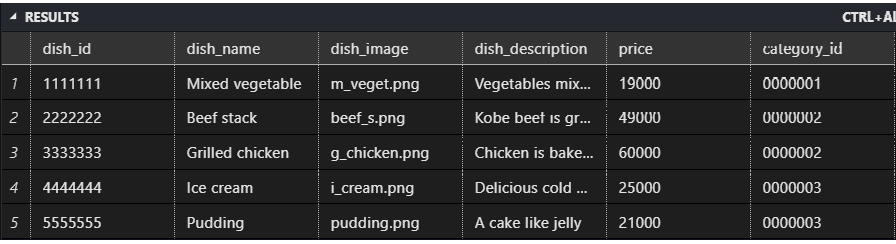
\includegraphics[width=10cm]{vitran/insert_dishes.png}
				\end{center}
			\end{figure}
			
			\subsubsection{Bảng "ORDER\_DISHES"}
			Đây là các lệnh dùng để thêm dữ liệu vào bảng "ORDER\_DISHES":
			\begin{lstlisting}				
				------------------------------------------------
				INSERT INTO ORDER_DISHES
				VALUES
				('1231231', null, null, '1111111', 'vitran', 'Unpaid', 157000, 'App', 'Ly Thuong Kiet', '0000001');
				INSERT INTO ORDER_DISHES
				VALUES
				('4564564', '2233445', '01112021', '1111111', 'vitran', 'Delivered', 330000, 'Live', 'Ly Thuong Kiet', null);
			\end{lstlisting}
			Để hiển thị dữ liệu trong bảng "ORDER\_DISHES", chúng ta chạy câu lệnh dưới đây:
			\begin{lstlisting}
				select * from ORDER_DISHES;
			\end{lstlisting}
			Sau khi thực hiện truy vấn, kết quả thu được là:
			\begin{figure}[h!]
				\begin{center}
					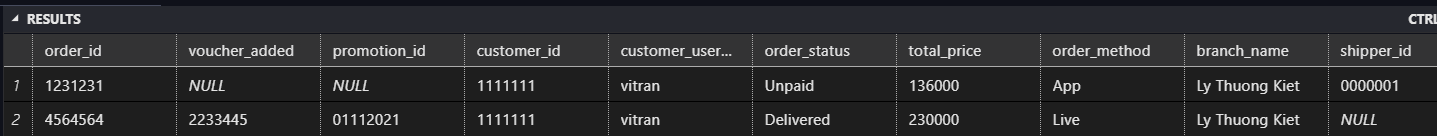
\includegraphics[width=10cm]{vitran/insert_od.png}
				\end{center}
			\end{figure}
		
			\subsubsection{Bảng "DISHES\_LIST"}
			Đây là các lệnh dùng để thêm dữ liệu vào bảng "DISHES\_LIST":
			\begin{lstlisting}				
				------------------------------------------------
				INSERT INTO DISHES_LIST
				VALUES
				('1231231', '1111111', 2);
				INSERT INTO DISHES_LIST
				VALUES
				('1231231', '2222222', 2);
				INSERT INTO DISHES_LIST
				VALUES
				('1231231', '5555555', 1);
				
				INSERT INTO DISHES_LIST
				VALUES
				('4564564', '1111111', 4);
				INSERT INTO DISHES_LIST
				VALUES
				('4564564', '2222222', 2);
				INSERT INTO DISHES_LIST
				VALUES
				('4564564', '3333333', 1);
				INSERT INTO DISHES_LIST
				VALUES
				('4564564', '4444444', 3);
				INSERT INTO DISHES_LIST
				VALUES
				('4564564', '5555555', 1);		
			\end{lstlisting}
			Để hiển thị dữ liệu trong bảng "DISHES\_LIST", chúng ta chạy câu lệnh dưới đây:
			\begin{lstlisting}
				select * from DISHES_LIST;
			\end{lstlisting}
			Sau khi thực hiện truy vấn, kết quả thu được là:
			\begin{figure}[h!]
				\begin{center}
					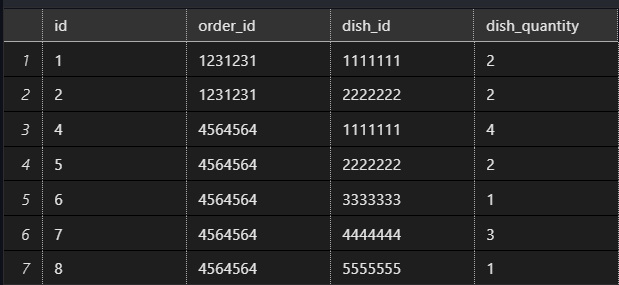
\includegraphics[width=10cm]{vitran/insert_dl.png}
				\end{center}
			\end{figure}
			
			\subsubsection{Bảng "ORDER\_BILLS"}
			Đây là các lệnh dùng để thêm dữ liệu vào bảng "ORDER\_BILLS":
			\begin{lstlisting}						
				------------------------------------------------
				INSERT INTO ORDER_BILLS
				VALUES
				('2021-11-20 19:00:34', 'Cash', 230000, '4564564');
			\end{lstlisting}
			Để hiển thị dữ liệu trong bảng "ORDER\_BILLS", chúng ta chạy câu lệnh dưới đây:
			\begin{lstlisting}
				select * from ORDER_BILLS;
			\end{lstlisting}
			Sau khi thực hiện truy vấn, kết quả thu được là:
			\begin{figure}[h!]
				\begin{center}
					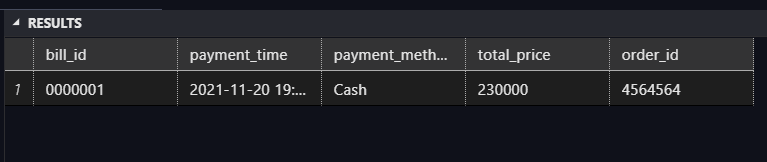
\includegraphics[width=10cm]{vitran/insert_ob.png}
				\end{center}
			\end{figure}
	\section{Phần riêng}
	\subsection{Thành viên 1}
	\begin{itemize}
		\item Họ tên: Trần Long Vĩ
		\item MSSV: 1814804
		\item DBMS: MSSQL server 
	\end{itemize}
	\subsubsection{Thủ tục Insert dữ liệu}
	\paragraph{Thủ tục Insert dữ liệu cho bảng "ORDER\_DISHES"\\}
	Chức năng của procedure này dùng để tạo một hàng trong bảng "ORDER\_DISHES".\\
	Câu lệnh tạo thủ tục:
	\begin{lstlisting}
		CREATE or alter PROCEDURE Insert_Tuple_2_ORDER_DISHES
		@order_id char(7),
		@voucher_added char(7),
		@customer_username varchar(50),
		@order_status char(10),
		@order_method char(10),
		@branch_name varchar(50),
		@shipper_id char(7)
		as
		begin
		DECLARE @flag AS int
		set @flag = 0
		IF @order_id=null 
		BEGIN
		RAISERROR ('Order ID must not equal "NULL"!', 16, 1)
		set @flag = -1
		END
		if @customer_username=null
		BEGIN
		RAISERROR ('Customer Username must not equal "NULL"!', 16, 1)
		set @flag = -1
		END
		if @order_status=null
		BEGIN
		RAISERROR ('Order status must not equal "NULL"!', 16, 1)
		set @flag = -1
		END
		if (@order_status != 'Unpaid' and @order_status != 'Paid' and @order_status!='Delivered' and @order_status!='Cancelled')
		BEGIN
		RAISERROR ('Invalid Order status value!', 16, 1)
		set @flag = -2
		END
		if @order_method=null
		BEGIN
		RAISERROR ('Last name must not equal "NULL"!', 16, 1)
		set @flag = -1
		END
		if (@order_method!='Live' and @order_method!='App' and @order_method!='Website')
		BEGIN
		RAISERROR ('Invalid Order method value!', 16, 1)
		set @flag =  -2
		END
		if @branch_name=null
		BEGIN
		RAISERROR ('Gender must not equal "NULL"!', 16, 1)
		set @flag =  -1
		END
		
		IF @flag=0
		BEGIN
		declare @promotion_id char(8);
		SET @promotion_id = (select promotion_id from VOUCHERS where voucher_id = @voucher_added);
		declare @customer_id char(7);
		set @customer_id = (select account_id from CUSTOMERS where username = @customer_username);
		INSERT INTO ORDER_DISHES
		VALUES
		(@order_id, @voucher_added, @promotion_id, @customer_id, @customer_username, @order_status, 0, @order_method, @branch_name, @shipper_id)
		END
		end;
	\end{lstlisting}
	Procedure này nhận vào 7 đối số ứng với $7/10$ thuộc tính trong bảng "ORDER\_DISHES". Ba thuộc tính còn lại bao gồm:
	\begin{itemize}
		\item "promotion\_id" là mã của sự kiện, sẽ được truy vấn trong bảng "VOUCHERS" dựa trên "voucher\_id" với điều kiện voucher đó chưa hết hạn.
		\item "customer\_id" là mã khách hàng, sẽ được truy vấn trong bảng "CUSTOMERS" dựa trên "customer\_username".
		\item "total\_price" là tổng số tiền khách hàng phải thanh toán. Giá trị này sẽ được cập nhật khi thêm các tuple tương ứng với "order\_id" vào bảng "DISHES\_LIST".
	\end{itemize}
	Câu lệnh thực thi thủ tục mẫu:
	\begin{lstlisting}
		exec Insert_Tuple_2_ORDER_DISHES 
		'4554443', null, 'vitran', 'Unpaid', "Live", "Ly Thuong Kiet", null;
	\end{lstlisting}
	Sau khi chạy, một tuple mới sẽ được thêm vào "ORDER\_DISHES" với $total\_price = 0$:
	\begin{figure}[h!]
		\begin{center}
			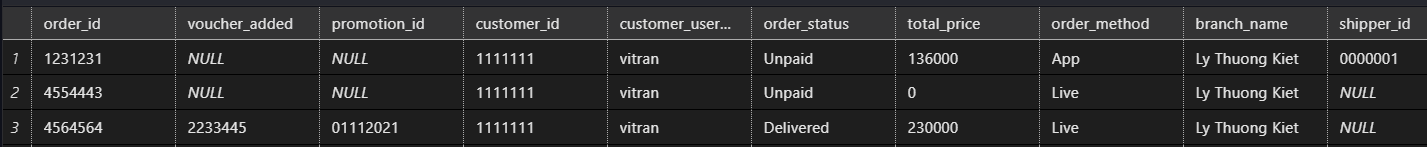
\includegraphics[width=10cm]{vitran/p_insert_od.png}
		\end{center}
	\end{figure}
	\paragraph{Thủ tục insert dữ liệu cho bảng "DISHES\_LIST"\\}
	Chức năng của procedure này dùng để tạo một hàng hoặc chỉnh sửa số lượng món ăn trong bảng "DISHES\_LIST". Tuple sẽ được chỉnh sửa nếu đã tồn tại tuple tương ứng, khi đó giá trị "dish\_quantity" sẽ được cập nhật dựa trên dữ liệu nhập vào.\\
	Câu lệnh tạo thủ tục:
	\begin{lstlisting}
		CREATE or alter PROCEDURE Insert_Tuple_2_DISHES_LIST
		@order_id char(7),
		@dish_id char(7),
		@dish_quantity int
		as
		begin
		DECLARE @flag AS int
		set @flag = 0
		IF @order_id=null 
		BEGIN
		RAISERROR ('Order ID must not equal "NULL"!', 16, 1)
		set @flag = -1
		END
		if @dish_id=null
		BEGIN
		RAISERROR ('Dish ID must not equal "NULL"!', 16, 1)
		set @flag =  -1
		END
		if @dish_quantity=null
		BEGIN
		RAISERROR ('Dish quantity must not equal "NULL"!', 16, 1)
		set @flag =  -1
		END
		if @dish_quantity < 0
		BEGIN
		RAISERROR ('Dish quantity must not equal "NULL"!', 16, 1)
		set @flag =  -1
		END
		
		IF @flag=0
		BEGIN
		if not exists(select * from DISHES_LIST where order_id = @order_id and dish_id = @dish_id)
		begin
		INSERT INTO DISHES_LIST
		VALUES
		(@order_id, @dish_id, @dish_quantity)
		end
		else
		BEGIN
		UPDATE DISHES_LIST 
		SET dish_quantity = @dish_quantity 
		where order_id = @order_id and dish_id = @dish_id;
		end
		END
		end;
	\end{lstlisting}
	Câu lệnh thực thi thủ tục mẫu:
	\begin{lstlisting}
		exec Insert_Tuple_2_DISHES_LIST '4564564', '5555555', 1;
		select * from DISHES_LIST;
	\end{lstlisting}
	Sau khi chạy, một tuple mới sẽ được thêm vào "DISHES\_LIST":
	\begin{figure}[h!]
		\begin{center}
			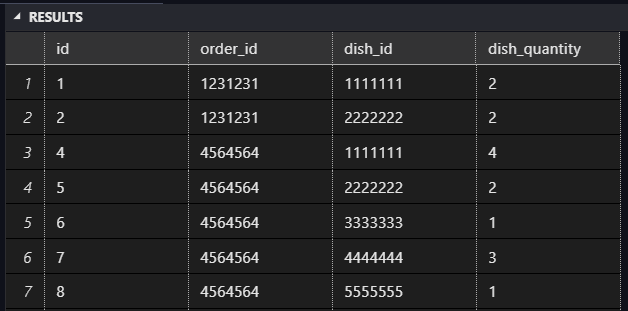
\includegraphics[width=10cm]{vitran/p_insert_dl.png}
		\end{center}
	\end{figure}
	\newpage
	Nếu tiếp tục chạy lệnh trên với giá trị "dish\_quantity" khác, ta sẽ thấy giá trị này thay đổi ở hàng tương ứng thay vì tạo một hàng mới:
	\begin{figure}[h!]
		\begin{center}
			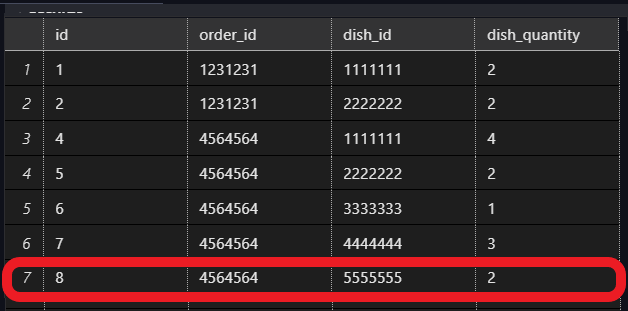
\includegraphics[width=10cm]{vitran/p_insert_dl1.png}
		\end{center}
	\end{figure}
	\subsubsection{Trigger}
	\paragraph{Trigger kiểm soát các hành động của bảng "DISHES\_LIST"\\}
	Trigger dùng để kiểm soát hành vi INSERT, DELETE và UPDATE trên bảng "DISHES\_LIST" có nhiệm vụ kiểm tra "order\_id" trong bảng "inserted" hoặc "deleted" tương ứng, nếu hợp lệ, sẽ tự động cập nhật lại giá trị "total\_price" trong bảng "ORDER\_DISHES". \\
	Câu lệnh tạo trigger:
	\begin{lstlisting}
		create or alter TRIGGER Insert_Update_DISH_LIST_trigger
		on DISHES_LIST
		after INSERT, UPDATE
		AS
		BEGIN
		DECLARE @order_id INT;
		SET @order_id = (select top 1 order_id from inserted);
		if @order_id is null
		BEGIN
		RAISERROR ('Order ID must not equal "NULL"!', 16, 1);
		ROLLBACK;
		end;
		declare @payment_price int;
		set @payment_price = (select dbo.cal_payment_price(@order_id));
		if @payment_price < 0 or @payment_price = null
		BEGIN
		RAISERROR ('Oups, something happened!', 16, 1);
		ROLLBACK;
		end;
		update ORDER_DISHES
		set total_price = @payment_price
		where order_id = @order_id;
		end
		go
		
		create or alter TRIGGER Delete_DISH_LIST_trigger
		on DISHES_LIST
		after DELETE
		AS
		BEGIN
		DECLARE @order_id INT;
		SET @order_id = (select top 1 order_id from deleted);
		if @order_id is null
		BEGIN
		RAISERROR ('Order ID must not equal "NULL"!', 16, 1);
		ROLLBACK;
		end;
		declare @payment_price int;
		set @payment_price = (select dbo.cal_payment_price(@order_id));
		if @payment_price < 0 or @payment_price is null
		BEGIN
		RAISERROR ('Oups, something happened!', 16, 1);
		ROLLBACK;
		end;
		update ORDER_DISHES
		set total_price = @payment_price
		where order_id = @order_id;
		end
		go
	\end{lstlisting}
	
	Để kiểm tra câu lệnh trên hoạt động, ta sử dụng procedure được giới thiệu ở phần trước để thêm tuple vào bảng "DISHES\_LIST", sau đó so sánh bảng dữ liệu trước và sau câu lệnh:
	\begin{lstlisting}
		exec Insert_Tuple_2_DISHES_LIST '4564564', '5555555', 1;
		select dl.order_id, dl.dish_id, total_price from DISHES_LIST dl, ORDER_DISHES od where od.order_id = '4564564' and dl.order_id = '4564564'; 
	\end{lstlisting}
	
	Kết quả thu được cho thấy giá trị "total\_price" trong bảng "ORDER\_DISHES" đã giảm xuống một ứng với món có id "5555555" và giá $21.000$đ:
	\begin{figure}[h!]
		\begin{center}
			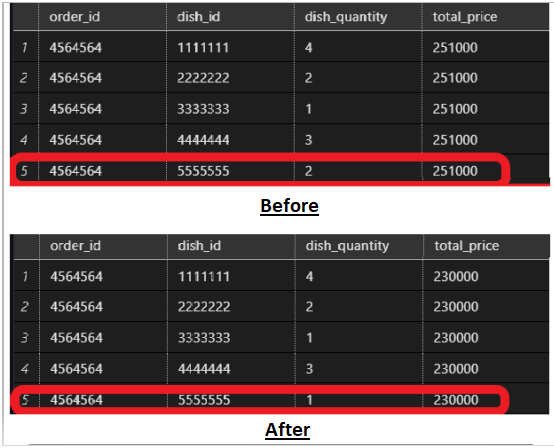
\includegraphics[width=10cm]{vitran/trigger_dl.png}
		\end{center}
	\end{figure}
	\newpage
	\paragraph{Trigger kiểm soát các hành động của bảng "ORDER\_DISHES"\\}
	Trigger này dùng để kiểm soát hành động INSERT, UPDATE của bảng "ORDER\_DISHES". Khi một tuple của bảng có giá trị "order\_status" được thiết lập ở giá trị "Paid" hoặc "Delivered":
	\begin{itemize}
		\item Bảng "ORDER\_BILLS" sẽ được INSERT thêm tuple mới tương ứng với "order\_id" vừa được INSERT hoặc UPDATE.
		\item Nếu tuple tương ứng được áp dụng voucher, giá trị voucher đó sẽ được chuyển thành "Used".
	\end{itemize}
	Câu lệnh tạo trigger:
	\begin{lstlisting}
		create or alter TRIGGER Update_ORDER_DISHES_trigger
		on ORDER_DISHES
		after INSERT, UPDATE
		AS
		BEGIN
		DECLARE @order_id INT;
		SET @order_id = (select order_id from inserted);
		if @order_id is null
		BEGIN
		RAISERROR ('Order ID must not equal "NULL"!', 16, 1);
		ROLLBACK;
		end;
		DECLARE @voucher_id char(7);
		set @voucher_id = (select voucher_added from ORDER_DISHES where order_id = @order_id);
		DECLARE @order_status CHAR(10);
		set @order_status = (select order_status from ORDER_DISHES where order_id = @order_id);
		if (@order_status='Paid' or @order_status='Delivered')
		begin
		if @voucher_id is not null
		begin
		DECLARE @voucher_status varchar(10);
		set @voucher_status = (select voucher_status from VOUCHERS where voucher_id = @voucher_id);
		if (@voucher_status != 'Expired')
		update VOUCHERS
		set voucher_status = 'Used'
		where voucher_id = @voucher_id;
		end
		if not exists (select * from ORDER_BILLS where order_id = @order_id)
		begin
		declare @datetime smalldatetime;
		set @datetime = (select CAST(GETDATE() AS smalldatetime));
		declare @price int;
		set @price = (select total_price
		from ORDER_DISHES
		where order_id = @order_id);
		insert into ORDER_BILLS
		values (@datetime, 'Cash', @price, @order_id);
		end;
		end;
		end
		go
	\end{lstlisting}
	Sau khi thực hiện tạo trigger, ta có thể test bằng cách thực hiện truy vấn tới 2 bảng "VOUCHERS" và "DISHES\_LIST" để kiểm tra sự thay đổi:
	\begin{lstlisting}
		-- UPDATE voucher status tester
		update ORDER_DISHES set order_status = 'Paid' where order_id = '4564564';
		select voucher_added, voucher_value, voucher_status from ORDER_DISHES od, VOUCHERS v
		where voucher_added = voucher_id;
		-- INSERT tuple to ORDER_BILLS tester
		update ORDER_DISHES set order_status = 'Paid' where order_id = '5067984';
		select * from ORDER_BILLS;
	\end{lstlisting}
	Kết quả thu được sau khi thực thi các lệnh truy vấn được mô tả dưới đây:
	\begin{figure}[h!]
		\begin{center}
			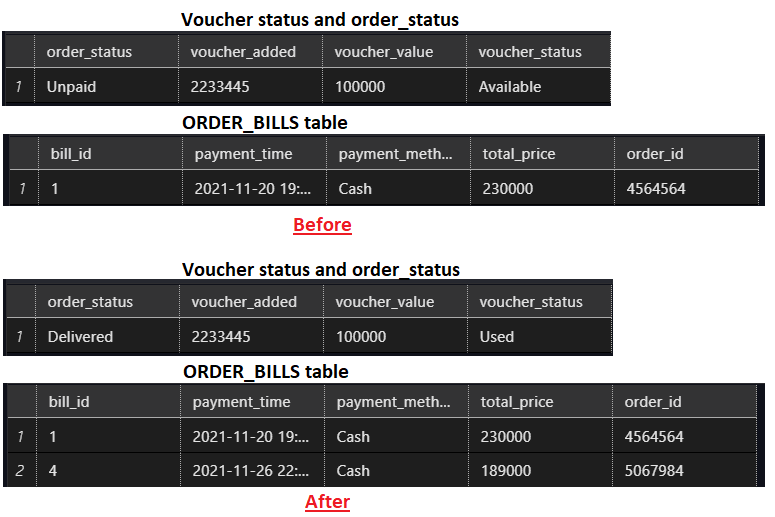
\includegraphics[width=10cm]{vitran/trigger_od.png}
		\end{center}
	\end{figure}
	\newpage
	\subsubsection{Thủ tục chứa câu SQL}
	\paragraph{Thủ tục truy vấn danh sách món ăn dựa trên order\_id\\}
	Thủ tục này được thiết kế nhằm mục đích truy vấn các thông tin về danh sách món ăn thuộc một đơn hàng, bao gồm các thông tin về tên món ăn, giá tiền, số lượng và tổng giá. Thủ tục nhận vào một đối số là "order\_id" là mã của đơn hàng cần truy vấn. \\
	Các câu lệnh dùng để tạo thủ tục:
	\begin{lstlisting}
		CREATE or alter PROCEDURE Display_dish_list_of_order
		@order_id char(7)
		as
		begin
		DECLARE @flag AS int
		set @flag = 0
		IF @order_id=null 
		BEGIN
		RAISERROR ('Order ID must not equal "NULL"!', 16, 1)
		set @flag = -1
		END
		
		IF @flag=0
		BEGIN
		select dish_name, price, dish_quantity, (price*dish_quantity) as 'Total price'
		from DISHES d, DISHES_LIST l
		where d.dish_id = l.dish_id and l.order_id = @order_id
		order by dish_quantity ASC
		END
		end;
	\end{lstlisting}
	Để thực thi thủ tục trên, ta thực hiện lệnh dưới đây (ở dưới đây là ví dụ áp dụng cho order\_id = '4564564'):
	\begin{lstlisting}
		exec Display_dish_list_of_order '4564564'; 
	\end{lstlisting}
	Sau khi thực thi lệnh trên, kết quả thu được là:
	\begin{figure}[h!]
		\begin{center}
			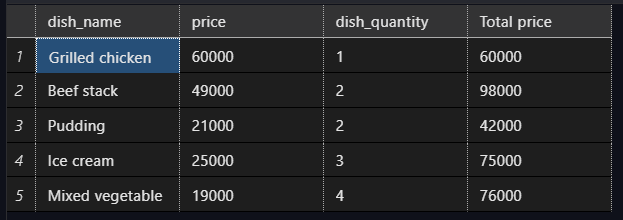
\includegraphics[width=10cm]{vitran/p_dl_d.png}
		\end{center}
	\end{figure}
	
	\paragraph{Thủ tục truy vấn các thông tin liên quan đến đơn hàng\\}
	Thủ tục này được thiết kế nhằm truy vấn các thông tin về mã đơn hàng, tên đăng nhập của khách hàng, giá gốc - giá thanh toán - giá được giảm cũng như các thông tin khác về hình thức thanh toán, trạng thái đơn hàng và chi nhánh đặt hàng. \\
	Các câu lệnh dùng để tạo thủ tục:
	\begin{lstlisting}
		CREATE or alter PROCEDURE Display_order_dishes_list
		as
		begin
		select dl.order_id, customer_username as 'username', 
		sum(price*dish_quantity) as 'o_price', total_price as 'p_price',
		dbo.cal_decreased_price(od.order_id) as 'd_price', 
		order_method, order_status, branch_name
		from DISHES_LIST dl, DISHES d, ORDER_DISHES od
		where dl.dish_id = d.dish_id and dl.order_id = od.order_id
		group by dl.order_id, customer_username, total_price, od.order_id, order_method, order_status, branch_name
		order by sum(price*dish_quantity) asc;
		end;
	\end{lstlisting}
	Sau khi khởi tạo, để thực thi thủ tục trên, ta chỉ cần thực thi câu lệnh dưới đây:
	\begin{lstlisting}
		exec Display_order_dishes_list;
	\end{lstlisting}
	Kết quả thu được là:
	\begin{figure}[h!]
		\begin{center}
			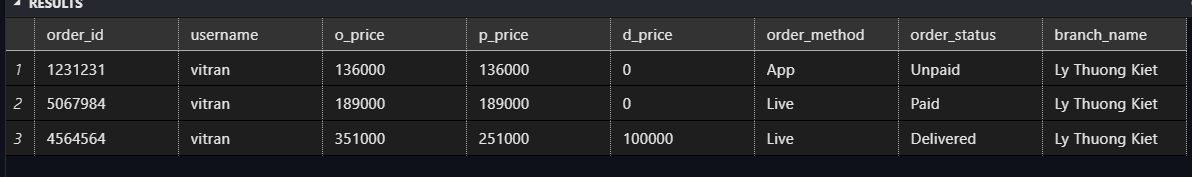
\includegraphics[width=10cm]{vitran/p_od_d_dl.png}
		\end{center}
	\end{figure}
	\subsubsection{Hàm}
	\paragraph{Hàm tính giá được giảm bởi voucher\\}
	Hàm được thiết kế với mục đích tính giá trị giảm của đơn hàng được áp dụng voucher. Hàm nhận vào mã đơn hàng và trả về kết quả bằng 0 nếu không có voucher, hoặc bằng giá trị của voucher nếu  voucher ID hợp lệ. \\
	Các câu lệnh dùng để tạo hàm
	\begin{lstlisting}
		create or alter function cal_decreased_price(@order_id char(7))
		returns INT
		AS
		BEGIN
		if @order_id is NULL
		return -1;
		DECLARE @voucher_id char(7);
		set @voucher_id = (select voucher_added	from ORDER_DISHES where order_id = @order_id);
		DECLARE @promotion_id char(8);
		set @promotion_id = (select promotion_id from order_dishes where order_id = @order_id);
		if (@voucher_id is NULL) or (@promotion_id is null)
		return 0;
		
		DECLARE @decreased_value int;
		set @decreased_value = (select voucher_value from VOUCHERS where voucher_id = @voucher_id and promotion_id = @promotion_id);
		if (@decreased_value is null) or (@decreased_value < 0)
		return -2;
		return @decreased_value
		end
	\end{lstlisting}
	Để thực thi và kiểm tra hàm, ta dùng câu lệnh dưới đây với mã đơn hàng là '4564564'(có áp dụng voucher) và '1231231'(không áp dụng voucher):
	\begin{lstlisting}
		select dbo.cal_decreased_price('4564564') as 'Order 4564564',
		dbo.cal_decreased_price('1231231') 'Order 1231231';
	\end{lstlisting}
	Sau khi thực thi lệnh, kết quả thu được là:
	\begin{figure}[h!]
		\begin{center}
			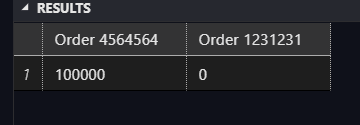
\includegraphics[width=10cm]{vitran/f_dp.png}
		\end{center}
	\end{figure}
	
	\paragraph{Hàm tính số tiền phải thanh toán\\}
	Hàm này được thiết kế để tính tổng số tiền phải thanh toán của một đơn hàng, với đối số nhận vào là mã đơn hàng đó. Hàm sau khi được thực thi sẽ truy vấn các giá trị liên quan để tính tổng giá gốc của đơn hàng và giá được giảm bởi voucher (nếu có), sau đó trả về tổng số tiền phải thanh toán. \\
	Các câu lệnh tạo hàm được hiển thị dưới đây:
	\begin{lstlisting}
		create or alter FUNCTION cal_payment_price(@order_id char(7))
		returns int
		AS
		BEGIN
		if @order_id is NULL
		return -1;
		declare @total_price INT;
		set @total_price = (select sum(price*dish_quantity) from DISHES d, DISHES_LIST l where l.order_id = @order_id and d.dish_id = l.dish_id);
		if @total_price is NULL
		return 0;
		declare @decreased_value int;
		set @decreased_value = (select dbo.cal_decreased_price(@order_id));
		if @decreased_value <= 0
		return @total_price;
		
		declare @payment_value int;
		set @payment_value = @total_price - @decreased_value;
		if @payment_value < 0
		return 0;
		return @payment_value;
		END
	\end{lstlisting}
	Để kiểm tra tính chính xác của hàm trên, ta có thể thực thi lệnh truy vấn dưới đây:
	\begin{lstlisting}
		select dl.order_id, dbo.cal_payment_price(od.order_id) as 'payment price', sum(price*dish_quantity) as 'original price', dbo.cal_decreased_price(od.order_id) as 'decreased price'
		from ORDER_DISHES od, DISHES_LIST dl, DISHES d
		where od.order_id = dl.order_id and dl.dish_id = d.dish_id
		group by od.order_id, dl.order_id;
	\end{lstlisting}
	Kết quả thu được là:
	\begin{figure}[h!]
		\begin{center}
			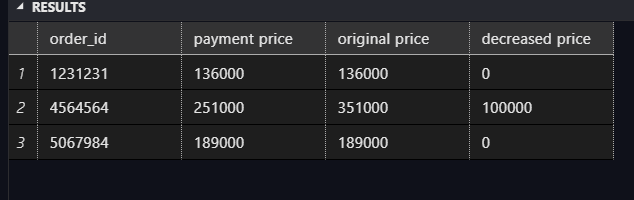
\includegraphics[width=10cm]{vitran/f_pp.png}
		\end{center}
	\end{figure}
	
	\subsubsection{Giao diện ứng dụng và các hình ảnh minh họa}
	Giao diện của ứng dụng là một bảng được liệt kê các mã đơn hàng và các thông tin liên quan tới mã đơn hàng đó. Dưới đây là hình ảnh giao diện của web:
	\begin{figure}[h!]
		\begin{center}
			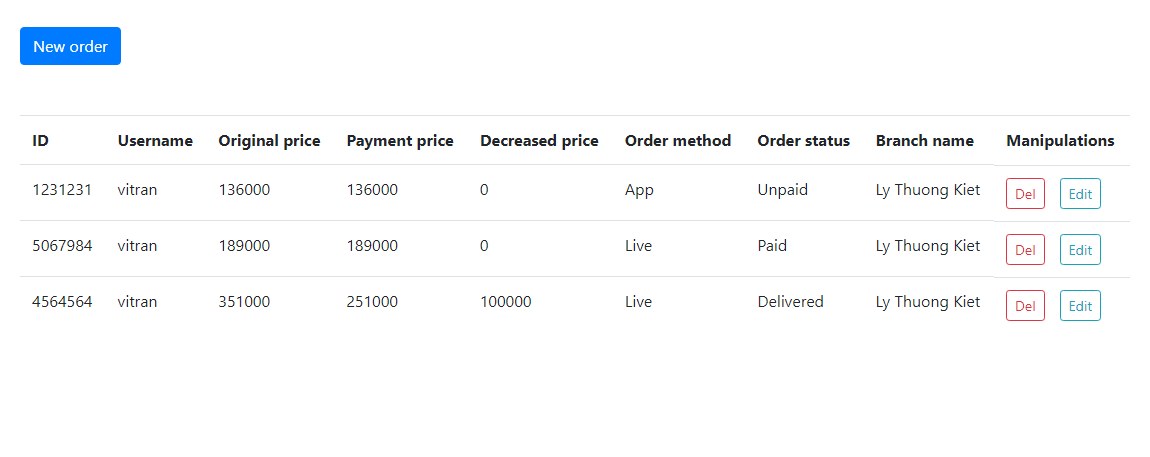
\includegraphics[width=10cm]{vitran/web_interface.png}
		\end{center}
	\end{figure}
	Trên giao diện của web, chúng ta có 3 nút thao tác:
	\begin{itemize}
		\item Nút dùng để thêm đơn hàng mới (New order): khi nút này được ấn, một form sẽ được hiển thị yêu cầu người dùng nhập các thông tin tương ứng để tạo đơn hàng.
		\begin{figure}[h!]
			\begin{center}
				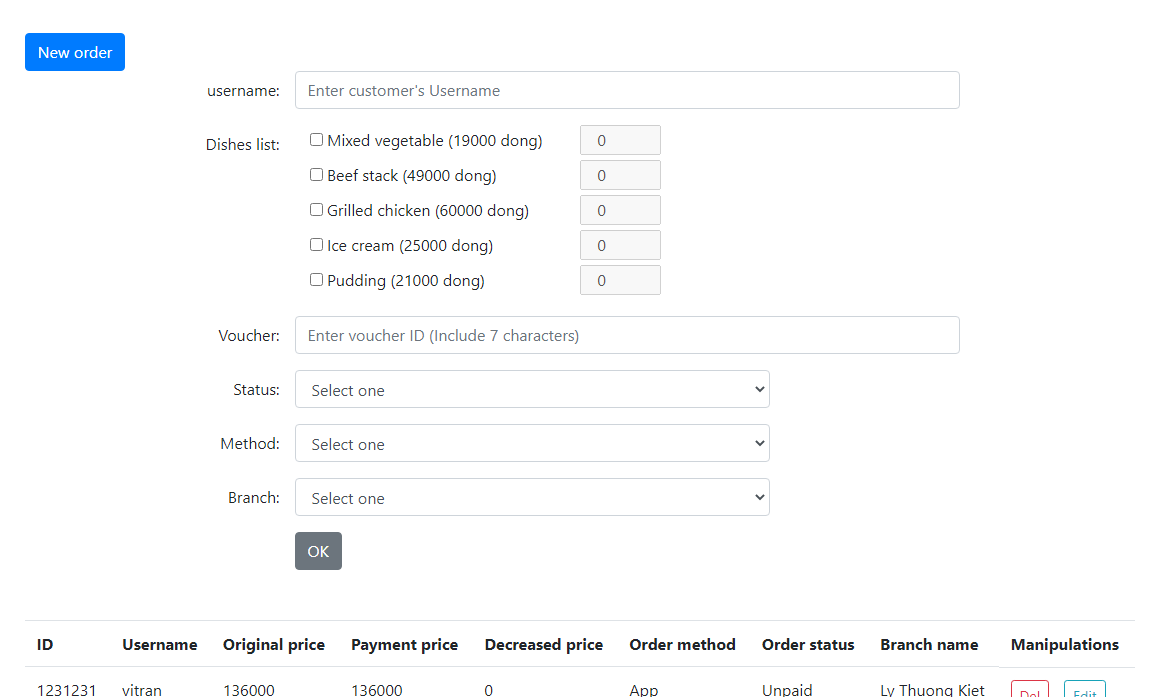
\includegraphics[width=10cm]{vitran/web_new_order.png}
			\end{center}
		\end{figure}
		Ở đây, các trường của form đều sẽ được kiểm tra dữ liệu trước khi được INSERT vào table. Cụ thể, có hai trường hợp lỗi, là lỗi về format nếu bỏ trống hoặc nhập sai trường dữ liệu (voucher có thể bỏ trống) hoặc lỗi không tồn tại nếu xét giá trị của username hoặc voucher. Tất cả các lỗi đều sẽ được thông báo ra màn hình chính dưới dạng chuỗi.
		\begin{figure}[h!]
			\begin{center}
				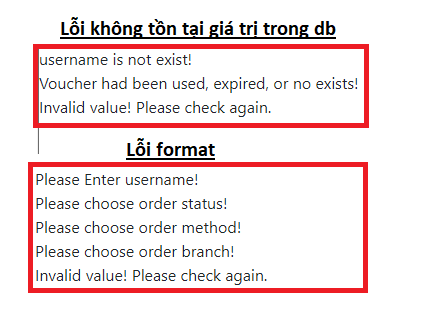
\includegraphics[width=10cm]{vitran/error_input.png}
			\end{center}
		\end{figure}
		\newpage
		Nếu dữ liệu nhập hợp lệ, đơn hàng mới sẽ được INSERT vào database và hiển thị lại ở bảng dưới.
		\begin{figure}[h!]
			\begin{center}
				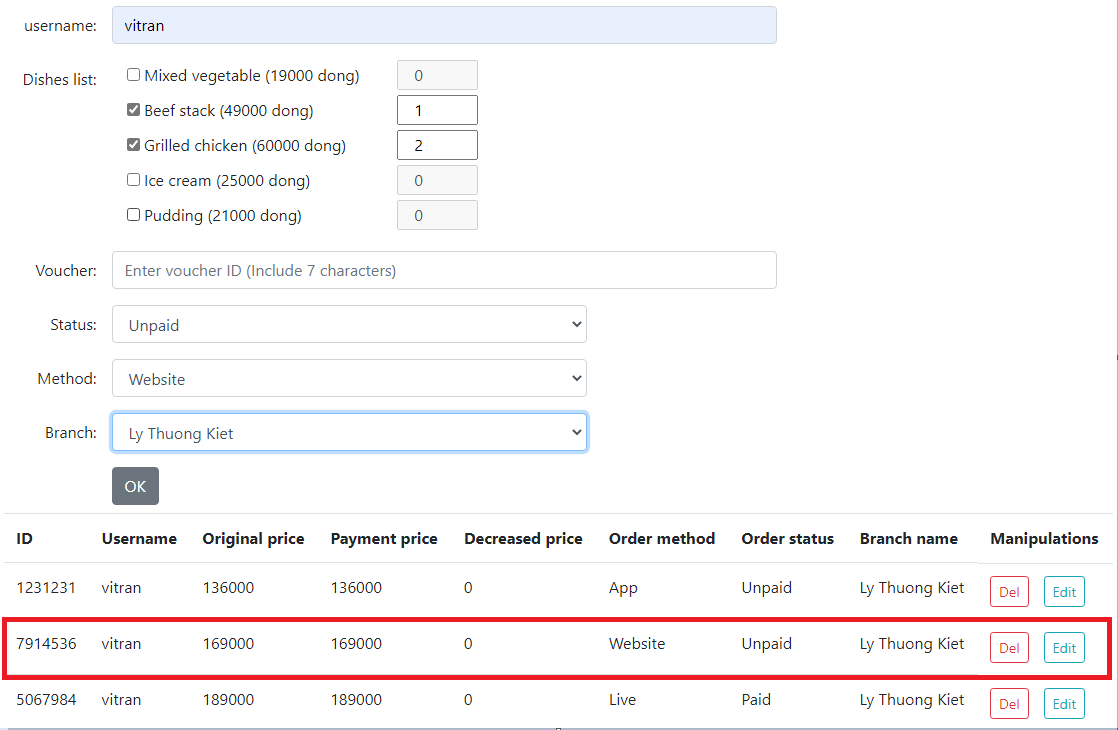
\includegraphics[width=10cm]{vitran/add_new.png}
			\end{center}
		\end{figure}
		
		\item Nút xóa được hiện ở cột Manipulations trong bảng, được dùng để xóa hàng tương ứng ra khỏi database.
		\begin{figure}[h!]
			\begin{center}
				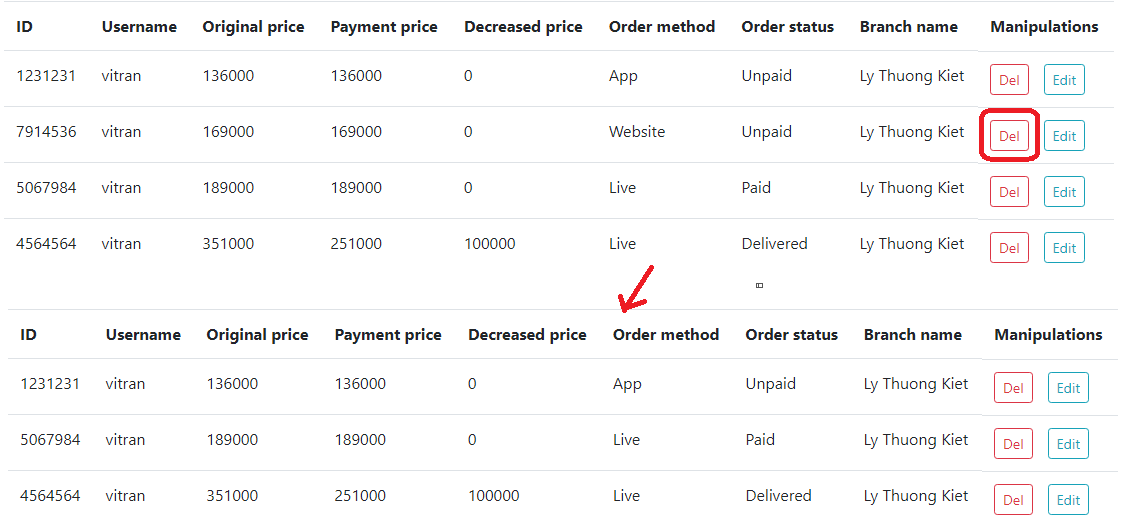
\includegraphics[width=10cm]{vitran/delete_row.png}
			\end{center}
		\end{figure}
		\newpage
		
		\item Nút Edit được hiện ở cột Manipulations trong bảng, được dùng để chỉnh sửa các giá trị của một đơn hàng. \\
		Khi nhấn vào nút này, trang sẽ tự chuyển hướng tới trang edit dùng để lấy các thông tin cần chỉnh sửa. Các trường thông tin ở đây đều sẽ kiểm tra đầu vào tương tự như tạo mới đơn hàng.
		\begin{figure}[h!]
			\begin{center}
				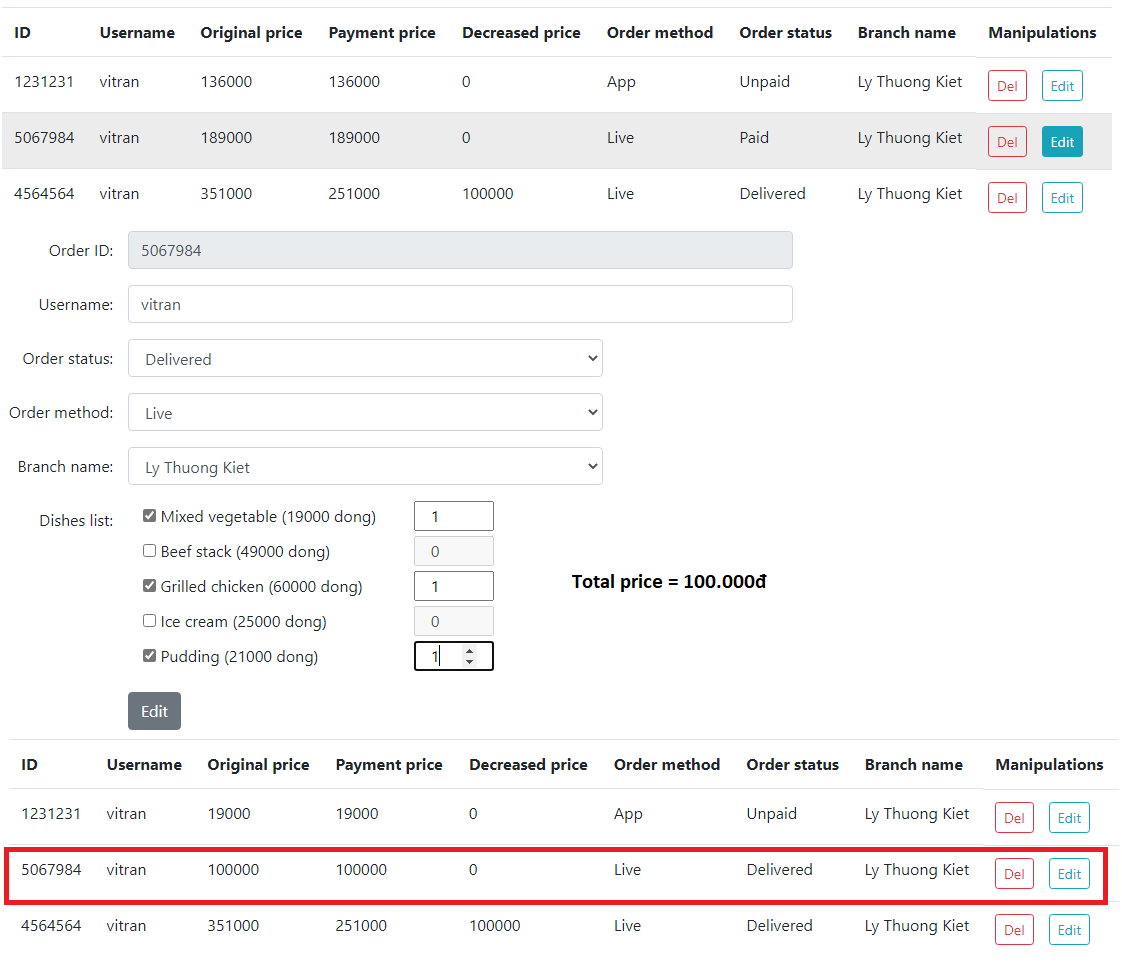
\includegraphics[width=10cm]{vitran/web_edit.png}
			\end{center}
		\end{figure}
		\newpage
	\end{itemize}
	$\dashrightarrow{lol}$
\end{document}